\documentclass[10pt]{article}
\usepackage[final]{graphicx}
\usepackage{amsfonts}
\usepackage{float} 

\topmargin -.5in
\textwidth 6.6in
\textheight 9in
\oddsidemargin 0in
\usepackage{color}
\newcommand{\arvind}[1]{{\color{red}{Arvind: {#1}}}}

\def\ds{\displaystyle}
\def\d{\partial}
\linespread{1.5}

\begin{document}
%%%%%%%%%%%%%%%%%%%%%%%%%%%%%%%%%%%%%%%%%%%
%%%%%%%Tuo1
To figure out whether we can use previous PM2.5 value to predict future PM2.5 value, we decide to conduct time series analysis. We focus our attention on the PM2.5 site which is located at latitude 33.79236 and longitude -118.175 ( It is really close to Long Beach). We collect monthly average PM2.5 values from Jan 2004 to Dec 2014 and plot them in figure 1 below.  

\begin{figure}[H]
\centering
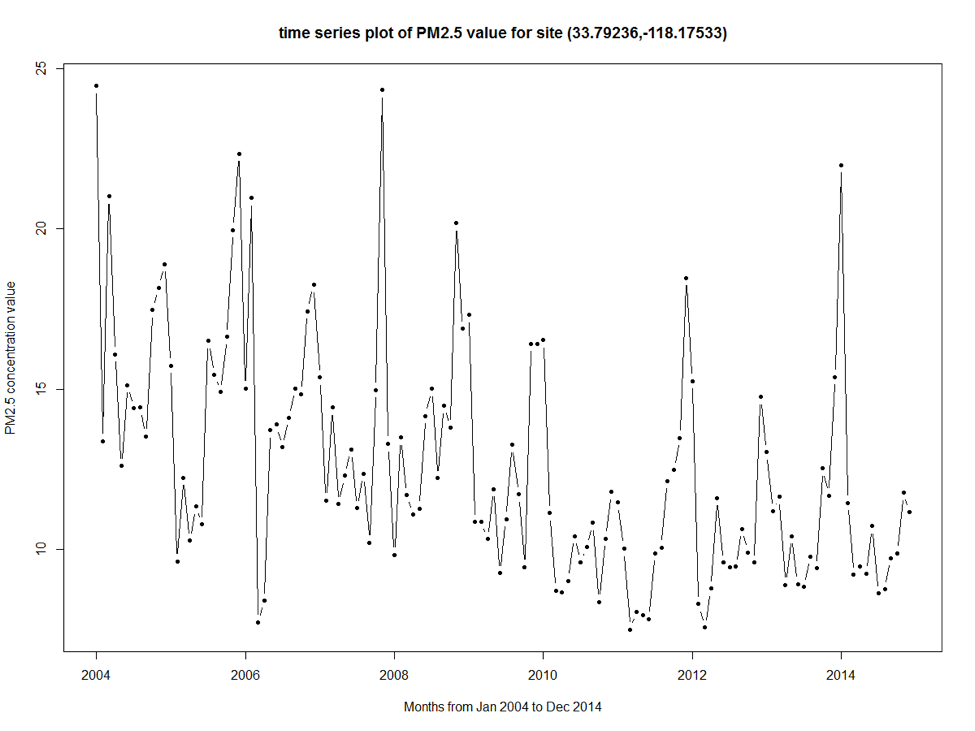
\includegraphics[width = 150mm]{ts1.png}
\caption{Time series plot of PM2.5 value for site (33.79236,	-118.17533)}
\label{graph4}
\end{figure}

There is a slightly downward trend over time about the time series and there seems to exist seasonality. We decide to use two different methods to fit the time series. One is Holt-Winters Exponential Smoothing. Exponential smoothing is a very popular scheme to produce a smoothed time series and it assigns exponentially decreasing weights as the observations get older(nist website). Holt-Winters Exponential Smoothing can be used to make short-term forecasts on a time series that can be described using an additive model with increasing or decreasing trend and seasonality(little book website). The second one is ARIMA model. ARIMA is the short for Autoregressive Integrated Moving Average. This model can be fitted to time series data either to better understand the data or to predict future points in the series(wikipedia website). For the ARIMA method, we firstly adjust the time series by subtracting the estimated seasonal component and then apply the model to the adjusted time series.

%%%%%%end_Tuo1
%%%%%%%%%%%%%%%%%%%%%%%%


%%%%%%%%%%%%%%%%%%%%%%Tuo 2

\subsubsection{Holt-Winters Exponential Smoothing}
We firstly draw fitted values plot based on Holt-Winters Exponential Smoothing. In figure 2, black line represents the variation of real PM values during 2004-2014 and red line represents the variation of fitted PM values during the period. We can see that although the two lines have similar trends, the fitted line is not accurate enough at many points.

\begin{figure}[H]
\centering
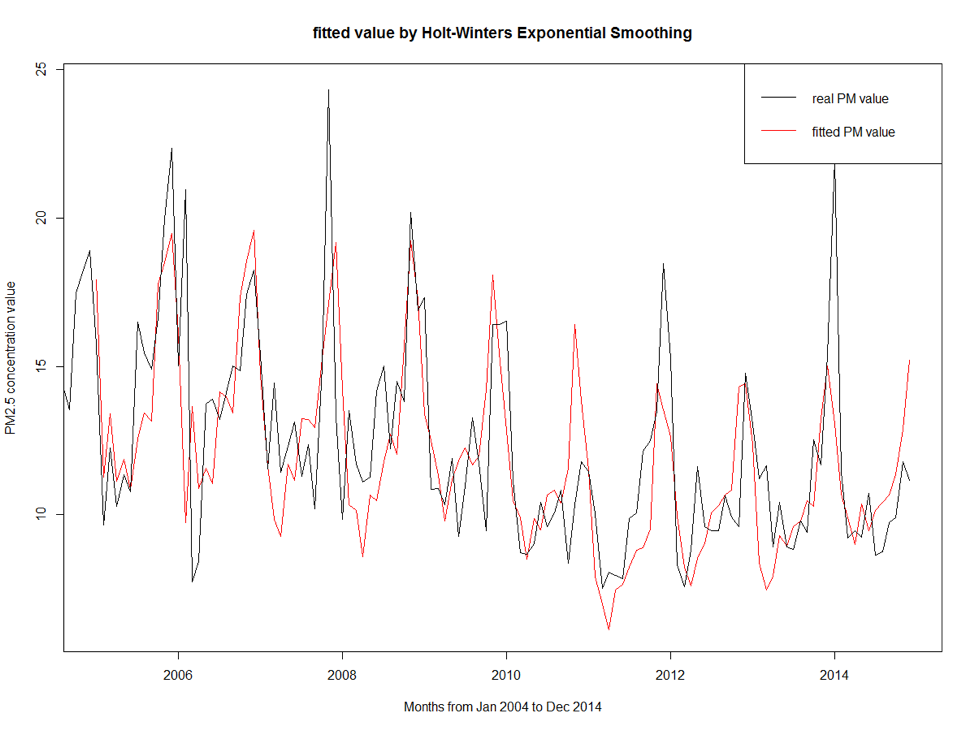
\includegraphics[width = 150mm]{ts2.png}
\caption{Fitted value by Holt-Winters Exponential Smoothing}
%\label{graph4}
\end{figure}

Then we predict PM2.5 values for the whole year 2015. In figure 3, the blue line represents the predicted values for 2015. The shadow of deep color represents the 80\% prediction interval for the predicted values and the shadow of light color represents the 95\% prediction interval for the predicted values.

\begin{figure}[ht!]
\centering
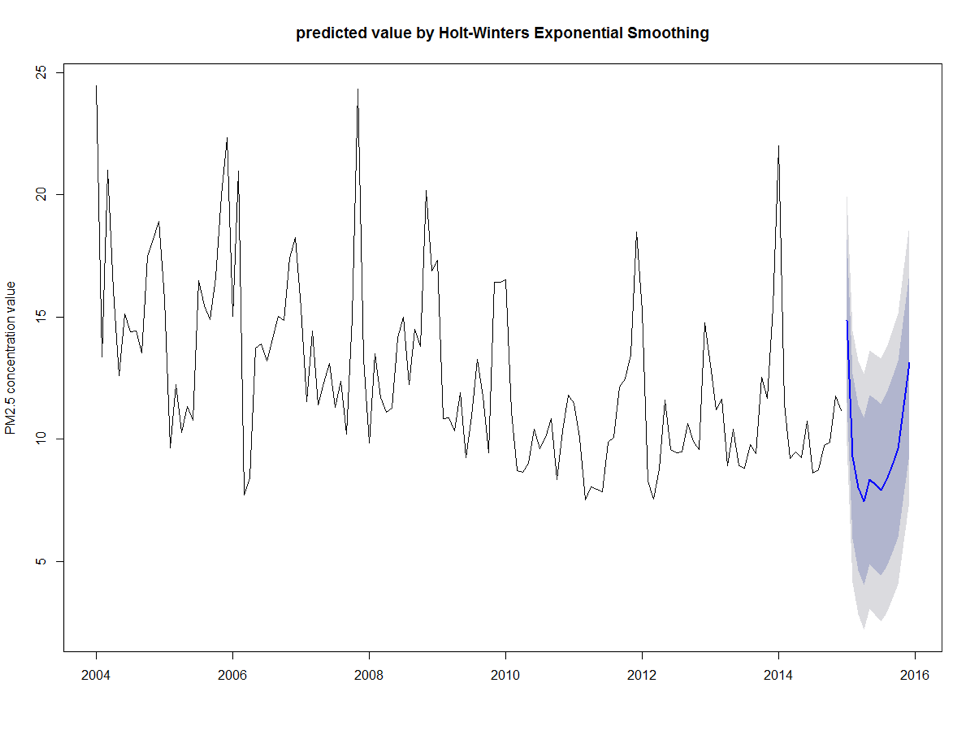
\includegraphics[width = 150mm]{ts3.png}
\caption{Predicted value by Holt-Winters Exponential Smoothin}
%\label{graph4}
\end{figure}

Now let us exmaine the effect of our prediction. We decide to use mean square error as our criterion. Lower mean square error indicates we have a better prediction. By comparing the predicted results and the real PM values for the year 2015, we find the mean square error between them is around 5.5. Becaues the mean of PM2.5 values during 2004-2014 is about 12.6, the mean square error is kind of large and this model is not very accurate.

\subsubsection{ARIMA model}
  Becaues there seems to exist seasonality in the PM2.5 time series, we want to decompose the time series and apply ARIMA model to the adjusted time series. We firstly decompose the PM2.5 time series and plot it. In figure 4, the four subplots respectively represent observed values, overall trend component, seasonal component and random part. From the seasonal component, we can see that there does exist differences among PM2.5 values in different months. By subtracting the seasonal component from the original time series, we get adjusted PM2.5 time series.

\begin{figure}[ht!]
\centering
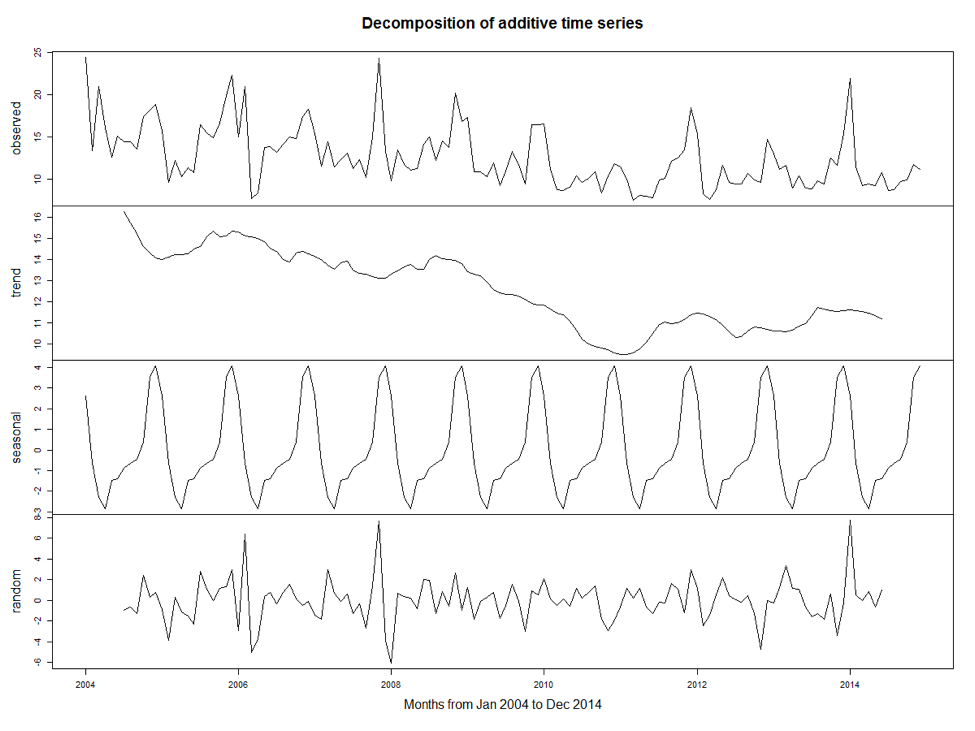
\includegraphics[width = 150mm]{ts4.png}
\caption{Decomposition of additive time series}
%\label{graph4}
\end{figure}

Then we draw fitted adjusted PM values based on ARIMA model in figure 5. The black line represents the variation of real adjusted PM values during 2004-2014  and red line represents the variation of fitted adjusted PM values during the period. From this plot we can see that the fitted line is really rough.

\begin{figure}[H]
\centering
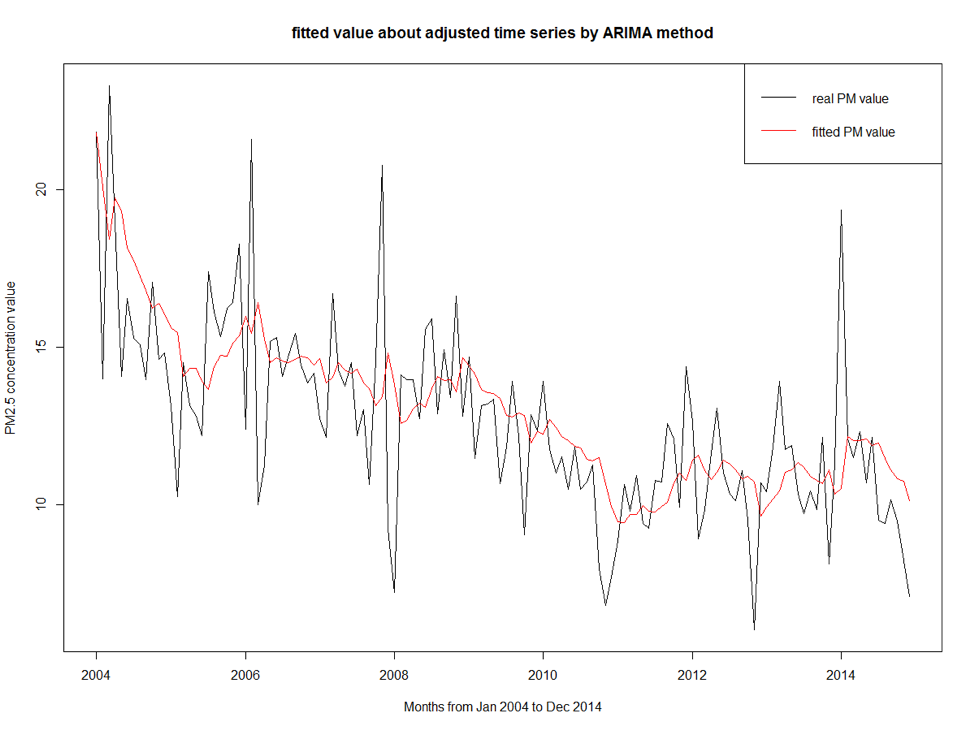
\includegraphics[width = 150mm]{ts5.png}
\caption{Fitted value about adjusted time series by ARIMA method}
%\label{graph4}
\end{figure}

Next, we predict the adjusted PM2.5 values for the whole year 2015. In figure 6, similarly as before, the blue line represents the predicted values for 2015. The shadow of deep color represents the 80\% prediction interval for the predicted values and the shadow of light color represents the 95\% prediction interval for the predicted values.

\begin{figure}[ht!]
\centering
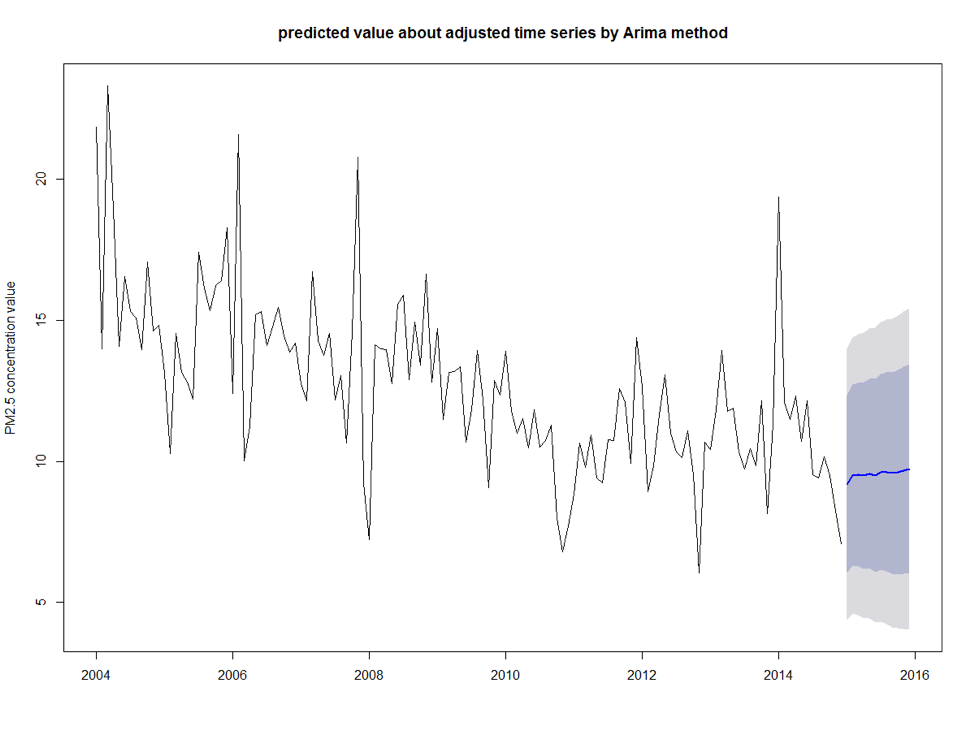
\includegraphics[width = 150mm]{ts6.png}
\caption{Predicted value about adjusted time series by Arima method}
%\label{graph4}
\end{figure}

Finally, we add seasonal component to our predicted results and then compare them with the real PM values during 2015. We find the mean square error is around 9.7 so we think the performance of ARIMA model is even not as good as Holt-Winters Exponential Smoothing.

In sum, the effect of prediction by time series is not very good. But it does give us some inspirations. For example, the PM 2.5 values will get different in different seasons. For next analytical step, we will combine PM2.5 values and some other corvariates to construct a better model.
%%%%%%%%%%%%%%%%% End Tuo2


%%%%%%%%%%%Put any citation 

%%% nist website:http://www.itl.nist.gov/div898/handbook/pmc/section4/pmc43.htm
%%% little book website: http://littlebookofrtimeseries-zh-cn.readthedocs.io/en/latest/src/timeseries.html#time-series-analysis
%%% wikipedia website: https://en.wikipedia.org/wiki/Autoregressive_integrated_moving_average

\end{document}










